\documentclass[11pt,a4paper]{article}
\usepackage[margin=2.6cm]{geometry}
\usepackage{amsmath,amssymb}
\usepackage{booktabs}
\usepackage{parskip}
\usepackage{pgfplots}
\pgfplotsset{compat=1.17}
\usepackage[colorlinks=true,linkcolor=black,urlcolor=blue]{hyperref}

\newcommand{\inkk}{\textbf{inkk}}

\title{\textbf{The inkk Human Score}\\[4pt]\large How it works, explained from zero}
\author{}
\date{}

\begin{document}
\maketitle

\section*{The one-sentence idea}

\inkk{} never judges the finished text. It watches \emph{the act of typing} and asks one question: \textbf{does this process look like a human being writing?}

A human leaves a mess while writing: irregular timing, pauses of every size, typos fixed two seconds later, sentences reworked. Pasted or machine-generated text leaves almost no process at all. The score measures the mess, in the best sense of the word.

\begin{center}
typing events $\to$ nine signals $\to$ evidence-weighted average $\to$ paste penalty $\to$ \textbf{score 0--100}
\end{center}

\section{What gets measured: nine signals}

While someone writes, the editor records small events: a key pressed, a key released, a character added, a deletion, the cursor moving. From that stream, nine signals are computed.

\begin{center}
\begin{tabular}{p{4.2cm} p{9.3cm}}
\toprule
\textbf{Signal} & \textbf{Plain-language meaning} \\
\midrule
Keystroke variance & The gaps between keystrokes. Humans are irregular; pasting has no gaps at all. \\
Key contact time & How long each key is physically held down. People vary; scripts do not. \\
Pause distribution & Real writing pauses at several scales: tiny hesitations, 2--10 second thinking pauses, longer breaks. \\
Corrections & Deletions and instant typo fixes. Humans typically delete 3--15\% of what they type. \\
Revisions & Jumping back into earlier text to rework it. \\
Bursts & Stretches of sustained, uninterrupted typing. \\
Rhythm cross-check & Irregular gaps \emph{and} varying key holds at the same time. Faking one without the other fails this. \\
Speed naturalness & Words per minute rises and falls over a session instead of holding one pace. \\
Engagement & Thinking pauses plus the share of time spent actively writing. \\
\bottomrule
\end{tabular}
\end{center}

\section{Every signal produces two numbers}

Each of the nine signals reports:

\begin{enumerate}
  \item \textbf{A value} $v$, between 0 and 1: \emph{``how human does this look?''}
  \item \textbf{A confidence} $c$, between 0 and 1: \emph{``how much evidence do I have?''}
\end{enumerate}

\subsection*{The value $v$: a soft switch}

Most values come from a \emph{sigmoid}, which is just a smooth switch. Below the human-typical level it outputs near 0, above it near 1, with a gentle slope in between instead of a hard cliff:

\begin{center}
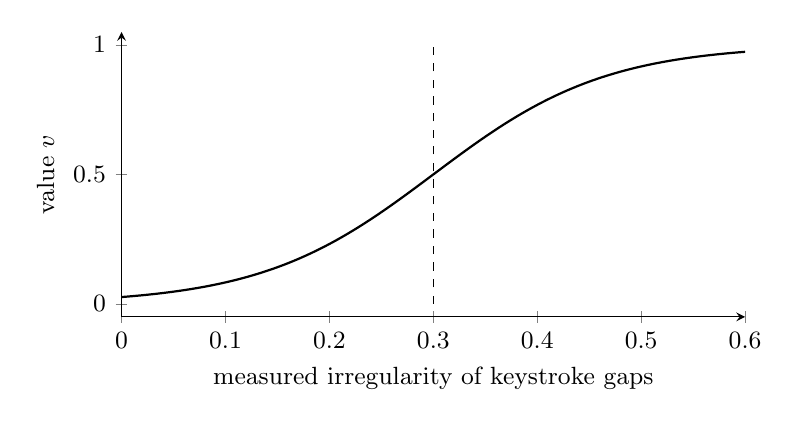
\begin{tikzpicture}
\begin{axis}[width=9.5cm,height=5.2cm,
  xlabel={measured irregularity of keystroke gaps},
  ylabel={value $v$},
  ymin=-0.05, ymax=1.05, xmin=0, xmax=0.6,
  axis lines=left, tick label style={font=\small}, label style={font=\small}]
\addplot[thick, domain=0:0.6, samples=120] {1/(1+exp(-12*(x-0.3)))};
\addplot[dashed] coordinates {(0.3,0) (0.3,1)};
\end{axis}
\end{tikzpicture}

\small (Illustrative shape. The dashed line marks the human-typical centre; each signal has its own centre and steepness.)
\end{center}

Written as a formula, for the keystroke-variance signal:
\[
v = \sigma\!\big(5 \cdot (\mathrm{CV} - 0.30)\big)
\qquad\text{where}\qquad
\sigma(x) = \frac{1}{1 + e^{-x}}
\]

In words: measure the irregularity of the typing gaps (CV). If it is above the human-typical centre of $0.30$, the value slides toward 1. If it is near zero (metronomic or pasted), the value slides toward 0.

\subsection*{The confidence $c$: an evidence ramp}

Confidence is even simpler. It is a straight ratio, capped at 1:
\[
c = \min\!\left(1,\; \frac{n}{N}\right)
\]

In words: ``I have seen $n$ pieces of evidence, and I need about $N$ before I fully trust this signal.'' For example: 18 keystroke gaps for variance, 10 key holds for contact time, 3 corrections for the corrections signal, roughly 40--60 words for the engagement and revision signals.

\textbf{Why confidence exists:} so that missing evidence is never treated as guilt. A short honest note, or typing on a phone (where key-hold times cannot be measured), simply leaves some signals silent. A silent signal does not vote at all; it neither helps nor hurts.

\section{Combining the nine signals}

The nine values are averaged, but not equally: each signal's vote is scaled by its importance $w$ (fixed weights, chosen by hand, summing to 1) and by its confidence $c$.

\[
\text{base} \;=\; \frac{\sum_{k=1}^{9} w_k \, c_k \, v_k}{\sum_{k=1}^{9} w_k \, c_k}
\]

Every symbol, in words:
\begin{itemize}
  \item $v_k$: how human signal $k$ looks (0 to 1)
  \item $c_k$: how much evidence signal $k$ has (0 to 1)
  \item $w_k$: how important signal $k$ is (variance 0.20, corrections 0.18, contact time 0.13, \dots)
  \item The top line adds up the weighted votes. The bottom line adds up the weight that actually voted. Dividing them gives the average of \emph{only the signals that had evidence}.
\end{itemize}

\section{The paste penalty}

Pasting up to 20\% of the content is treated as normal (quotes, links). Beyond that, the whole score is multiplied down:

\[
P(p) =
\begin{cases}
1 & p \le 0.2 \\[2pt]
1 - \dfrac{p - 0.2}{0.6} & 0.2 < p < 0.8 \\[6pt]
\approx 0 & p \ge 0.8
\end{cases}
\qquad p = \text{fraction of content that was pasted}
\]

Because this is a \emph{multiplier} on the final result, heavy pasting cannot be buried under a pile of typed filler. Half-pasted work caps the score at half.

\section{The full formula}

\[
\boxed{\;\text{score} \;=\; 100 \;\times\; P(p) \;\times\; \frac{\sum_k w_k \, c_k \, v_k}{\sum_k w_k \, c_k}\;}
\]

Plain-English translation: \textbf{the score is the average of how human each signal looks, where each signal's vote counts only as much as its evidence, times a penalty if too much was pasted.}

Two side quantities come from the same pieces:
\[
\text{confidence} = \sum_k w_k c_k
\qquad\text{(how much of the total voting weight actually fired)}
\]
which gates the label shown to readers (below 0.15 the piece is marked \emph{Faint}: not judged, just not enough evidence), and the per-signal contributions $w_k c_k v_k$, which are what the app lists as ``top contributors.''

\section{A worked example}

Someone types a short paragraph on a phone. Only three signals gather evidence (phones expose no key-hold times, so contact time stays silent):

\begin{center}
\begin{tabular}{lcccc}
\toprule
\textbf{Signal} & $w$ & $c$ & $v$ & $w \cdot c \cdot v$ \\
\midrule
Keystroke variance & 0.20 & 1.00 & 0.80 & 0.160 \\
Corrections        & 0.18 & 0.67 & 0.60 & 0.072 \\
Key contact time   & 0.13 & 0.00 & --   & 0.000 \\
\bottomrule
\end{tabular}
\end{center}

\[
\text{base} = \frac{0.160 + 0.072}{0.20 \cdot 1.00 + 0.18 \cdot 0.67} = \frac{0.232}{0.321} \approx 0.72
\]

Only 5\% of the content was pasted, so $P = 1$, and:
\[
\text{score} = 100 \times 1 \times 0.72 = \mathbf{72}
\]

Note what did \emph{not} happen: the missing contact-time signal did not drag the score down. It simply did not vote.

\section{Version 2: the learned fingerprint}

The formula above is a hand-built model: nine features chosen by a person, weights guessed by a person. Version 2 replaces the hand-picking with learning, once the stored writing sessions (the event batches) are numerous enough to train on.

\subsection*{The idea, with a map}

Imagine a huge map. Every writing session becomes \textbf{one dot} on that map. The \emph{encoder} is the mapmaker: it reads the whole event sequence and decides where the dot goes.

\[
z = f_\theta(e_1, e_2, \ldots, e_T)
\]

In words:
\begin{itemize}
  \item $e_1, \ldots, e_T$: the session's events in order (what happened + the time gap since the previous event), read like words in a sentence
  \item $f_\theta$: the encoder, a small neural network that reads sequences; $\theta$ is its adjustable knobs
  \item $z$: the dot. A list of numbers (a coordinate) summarising the session's entire \emph{style of being typed}. This is the writing-process fingerprint.
\end{itemize}

The goal of training: \textbf{all genuinely human sessions should land in the same region of the map}, and scripted, replayed, or synthetic typing should land visibly elsewhere.

\subsection*{How the mapmaker is trained: spot the sibling}

Training is a game played millions of times. Take two windows cut from the \emph{same} writer's session; call one the anchor and one the sibling. Mix the sibling into a line-up of windows from many \emph{other} writers. The mapmaker wins if the anchor's nearest dot in the line-up is its sibling.

\[
\mathcal{L} = -\log \frac{\exp\!\big(\mathrm{sim}(z_i, z_i^{+}) / \tau\big)}{\sum_{j} \exp\!\big(\mathrm{sim}(z_i, z_j) / \tau\big)}
\]

Every symbol, in words:
\begin{itemize}
  \item $z_i$: the anchor's dot; $z_i^{+}$: the sibling's dot; $z_j$: every dot in the line-up
  \item $\mathrm{sim}(\cdot,\cdot)$: how close two dots are (cosine similarity)
  \item $\tau$: a strictness dial for the game
  \item $\mathcal{L}$: the penalty. It is small when the sibling is clearly the closest match, large when it is not. Training nudges the knobs $\theta$ to shrink this penalty.
\end{itemize}

The consequence: sessions that share a real human process end up close together on the map. The mapmaker discovers \emph{its own} signals for this, hundreds of them, instead of using nine chosen by hand.

\subsection*{Scoring a new session}

Encode the session into its dot $z$, then ask how deep inside the human region it lies. The simplest version is a smooth boundary drawn across the map:

\[
\text{score} = \sigma(\mathbf{w} \cdot z + b) \;=\; \text{probability the process was human}
\]

In words: $\mathbf{w}$ and $b$ define the boundary line, $\mathbf{w} \cdot z + b$ measures which side of it the dot falls on and how far, and $\sigma$ (the same soft switch as before) turns that distance into a probability.

\subsection*{Why version 2 is harder to fool}

Version 1 checks nine known dials, so a determined spoofer knows exactly what to fake. Version 2 checks the \emph{joint shape of everything at once}, with signals no one published. To place a fake dot deep inside the human region, you would have to reproduce the full statistical texture of a human writing session. At that point, the easiest known method is: write it like a human.

\subsection*{How version 1 feeds version 2}

Version 1 is not throwaway. It provides trust from day one, and its scores label the accumulating sessions. Those labelled event batches are exactly the training data version 2 needs. The heuristic bootstraps the model that replaces it.

\end{document}
